\documentclass[12pt, openany]{report}
\usepackage[utf8]{inputenc}
\usepackage[T1]{fontenc}
\usepackage{amsmath,amsfonts,amssymb}
\usepackage{amssymb}
\usepackage{multicol}
\usepackage[a4paper,left=2.5cm,right=2.5cm,top=2.5cm,bottom=2.5cm]{geometry}
\usepackage[english]{babel}
\usepackage{libertine}
\usepackage{graphicx}
\usepackage{wrapfig}
\usepackage{amsthm}
\usepackage{float}
\usepackage{enumitem}
\usepackage{pythonhighlight}
\usepackage[]{titletoc}
\usepackage{empheq}
\usepackage{titlesec}
\usepackage{mathpazo}
\usepackage{xfrac}
\usepackage{textcomp}
\usepackage{mathtools}
\usepackage{hyperref}
\usepackage{caption}
\usepackage{tabularray}
\usepackage{subcaption}
\usepackage[bottom]{footmisc}
\usepackage{pdfpages}
\usepackage{tabularx}
\usepackage[skins]{tcolorbox}

\theoremstyle{definition}
\newtheorem{thm}{Theorem}[chapter]
\newtheorem{definition}[thm]{Definition}
\newtheorem{exmp}[thm]{Example} 
\newtheorem{lem}[thm]{Lemma}
\newtheorem{crl}[thm]{Corollary}

\titleformat{\chapter}[display]
  {\normalfont\bfseries}{}{0pt}{\Huge}
\newcommand{\hsp}{\hspace{20pt}}
\newcommand{\HRule}{\rule{\linewidth}{0.5mm}}
\newcommand\independent{\protect\mathpalette{\protect\independenT}{\perp}}
\def\independenT#1#2{\mathrel{\rlap{$#1#2$}\mkern2mu{#1#2}}}
\newcommand{\R}{\mathbb{R}}
\newcommand{\C}{\mathbb{C}}
% Define a new tcolorbox style with a red border and transparent interior
\tcbset{
    redbox/.style={
        enhanced,
        colframe=red,
        colback=white,
        boxrule=1pt,
        sharp corners,
        before skip=10pt,
        after skip=10pt,
        box align=center,
        width=\linewidth-2pt, % Adjust the width dynamically
    }
}
\newcommand{\boxedeq}[1]{
\begin{tcolorbox}[redbox]
    \begin{align}
        #1
    \end{align}
\end{tcolorbox}
}

\hbadness=100000
\begin{document}
\begin{titlepage}
    \begin{sffamily}
    \begin{center}
        
\includegraphics[scale=0.25]{img/page_de_garde.png} \\[1cm]
        \HRule \\[0.4cm]
        { \huge \bfseries LINMA2171 Numerical Analysis \\[0.4cm] }
    
        \HRule \\[1.5cm]
        \textsc{\LARGE Simon Desmidt}\\[1cm]
        \vfill
        \vspace{2cm}
        {\large Academic year 2024-2025 - Q1}
        \vspace{0.4cm}
         
        
\includegraphics[width=0.15\textwidth]{img/epl.png}
        
        UCLouvain\\
    
    \end{center}
    \end{sffamily}
\end{titlepage}

\setcounter{tocdepth}{1}
\tableofcontents
\chapter{Polynomials}
\(\mathcal{P}_n\) is the set of all real polynomials of degree at most \(n\). 
\begin{itemize}
    \item The Runge phenomenon is the explosion of the polynomial near the boundary of the domain when the interpolation points are chosen to be equidistant. A solution to that is to put more points near the boundary and less in the middle of the domain, e.g. Chebyshev points.
\end{itemize}
\section{Lagrange interpolation}
Let \(x_0,\dots,x_n\) be distinct real numbers. The Lagrange polynomial \(L_k\) of degree \(n\) is such that it is equal to 0 for all \(x_i\), \(i\neq k\) and \(1\) for \(x_k\). This serves as a base for the next interpolations. The general formula for the Lagrange polynomial is 
\begin{equation}
    L_k(x) = \prod_{i=0\\i\neq k}^n \frac{x-x_i}{x_k-x_i}\qquad k=0,1,\dots,n
\end{equation}
\begin{itemize}
    \item N.B.: we usually denote \(L_k(x;x_0,\dots,x_n)\) or let \(\chi = (x_0,\dots,x_n)\) and \(L_k(x;\chi)\). 
\end{itemize}
\section{Hermite interpolation}
Let \(x_0,\dots,x_n\) be distinct real numbers. Then, given two sets of real numbers \((y_0,\dots y_n)\) and \((z_0,\dots,z_n)\), there is a unique polynomial \(p_{2n+1}\in \mathcal{P}_{2n+1}\) such that 
\begin{equation}
    p_{2n+1} (x_i) = y_i \qquad p_{2n+1}'(x_i) =z_i \qquad i=0,\dots,n
\end{equation}
The polynomial \(p_{2n+1}\) is termed the Hermite interpolation polynomial of degree at most \(2n+1\) for the data points \((x_0,y_0,z_0),\dots,(x_n,y_n,z_n)\). The expression is 
\begin{equation}
    p_{2n+1}(x) = \sum_{k=0}^n \left(H_k(x)y_k + K_k(x)z_k\right) \qquad \begin{cases}
        H_k(x) = (L_k(x))^2(1-2L'_k(x_k)(x-x_k))\\
        K_k(x) = (L_k(x))^2(x-x_k)
    \end{cases}
\end{equation}
where \(L_k(x)\) is the Lagrange polynomial.
\begin{itemize}
    \item The \(H_k(x)\) are such that their derivative is zero for all \(x_i\), and their value is zero for all \(x_i\) except \(x_k\), where it is 1.\[H_k(x_i) = \delta_{ik}\qquad H_k'(x_i) = 0 \qquad \forall i\]
    \item The \(K_k(x)\) are such that their derivative is zero for all \(x_i\) except \(x_k\) where it is one, and their value is zero for all \(x_i\).\[K_k(x_i) = 0\qquad K_k'(x_i) = \delta_{ik} \qquad \forall i\]
\end{itemize}
\section{Neville's algorithm}
Let us assume we are given a set of support points \((x_i,y_i)\), \(i=0,1,\dots,n\), and \(p_n\) is their Lagrange interpolation polynomial. Let us now define the notation \(P_{i_0i_1\dots i_k}\in \mathcal{P}_k\), the polynomial for which \(P_{i_0i_1\dots i_k}(x_{i_j})=y_{i_j}\)  for all \(j=0,1,\dots,k\). We work by recursion, with the following formula:
\begin{equation}
    \begin{cases}
        P_i(x) = y_i\\
        P_{i_0i_1\dots i_k} = \frac{(x-x_{i_0})P_{i_1i_2\dots i_k}(x) - (x-x_{i_k})P_{i_0i_1\dots i_{k-1}}(x)}{x_{i_k}-x_{i_0}}
    \end{cases}
\end{equation}
Example:\\
Let us have four points \((x_0,y_0),\dots(x_3,y_3)\). We want the polynomial interpolating all of them, using Neville's algorithm. 
\begin{figure}[H]
    \centering
    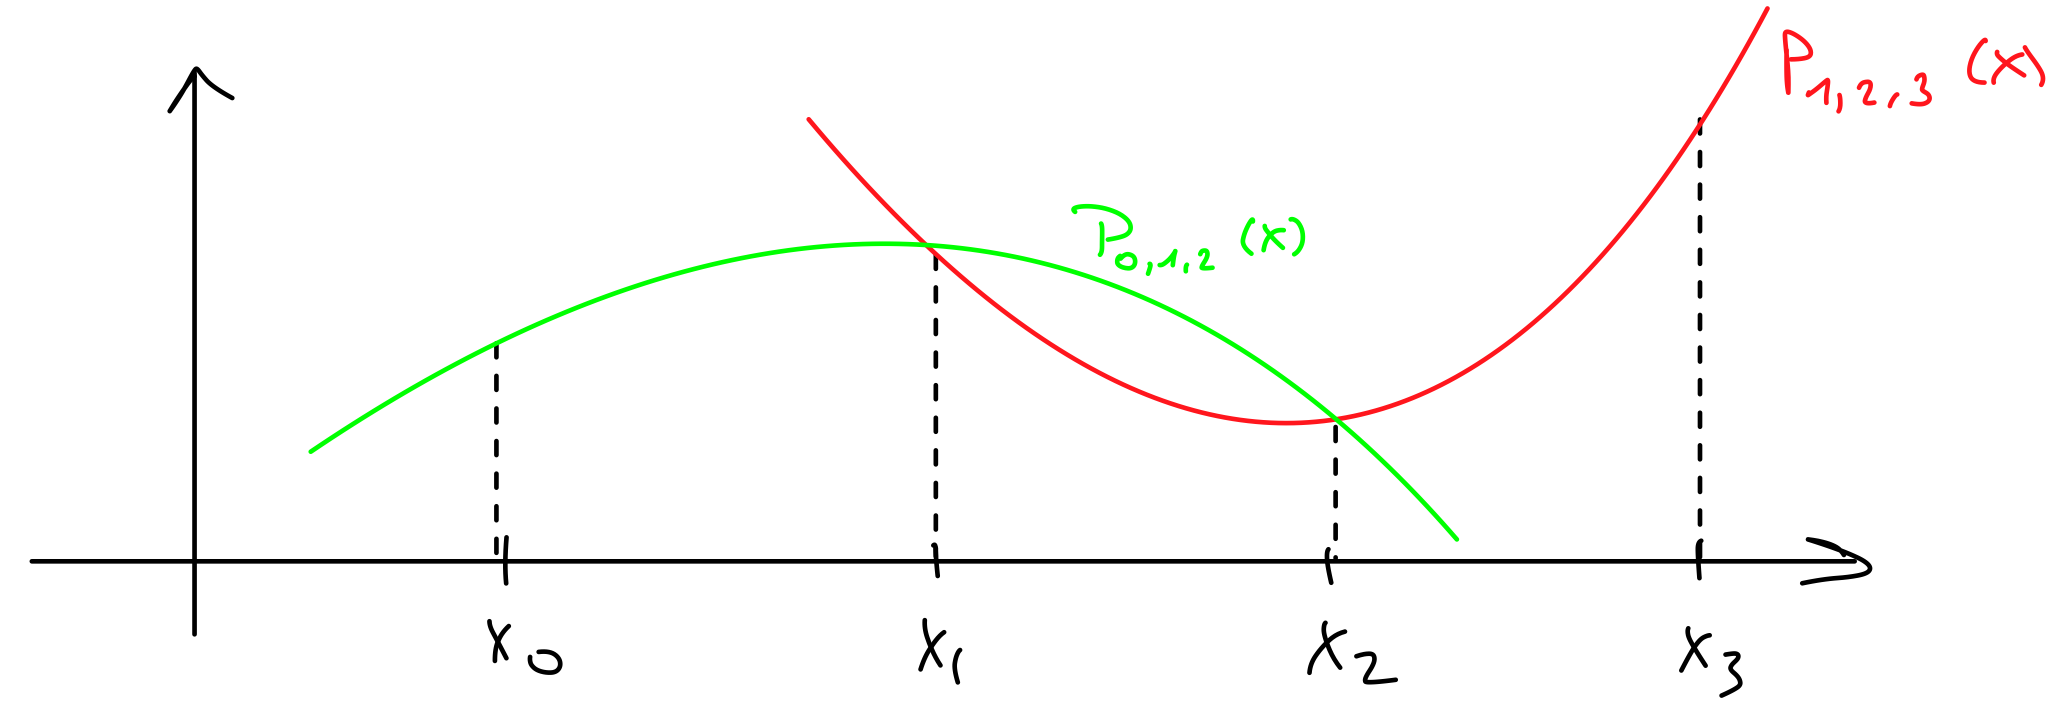
\includegraphics[width=0.5\linewidth]{img/neville.png}
\end{figure}
Here, 
\begin{equation}
    P_{0123}(x) = \frac{x-x_0}{x_3-x_0}\color{red}P_{123}(x)\color{black}+\frac{x_3-x}{x_3-x_0}\color{green}P_{012}(x)\color{black}
\end{equation}
\section{Newton's interpolation formula}
Newton's interpolation formula is used to evaluate polynomials with a computer, as it only needs to compute each operation \((x-x_i)\) one time. We write it like:
\begin{equation}
    p_n(x) = \left(\left(\dots\left(y_{0\dots n}(x-x_n)+y_{0\dots n-1}\right)(x-x_{n-1})+y_{0\dots n-2}\right)(x-x_{n-2})+\dots\right) + y_0
\end{equation}
And the recursive formula is
\begin{equation}
    P_{i_0i_1\dots i_k}= P_{i_0i_1\dots i_{k-1}}(x) + y_{i_0i_1\dots i_k}(x-x_{i_0})(x-x_{i_1})\dots(x-x_{i_{k-1}})
\end{equation}
\section{Linear algebra approach}
Let \((\phi_0,\dots,\phi_n)\) ba a basis of \(\mathcal{P}_n\), which is known to be an \((n+1)\)-dimensional linear space. The interpolation polynomial can thus be expressed in a unique way in the basis:
\begin{equation}
    p_n(x) = \sum_{i=0}^n a_i\phi_i(x)
\end{equation}
and the coefficient are obtained by solving the linear system
\begin{equation}
    \begin{bmatrix}
        \phi_0(x_0) & \phi_1(x_0) & \dots & \phi_n(x_0)\\
        \phi_0(x_1) & \phi_1(x_1) & \dots & \phi_n(x_1)\\
        \vdots  & \vdots & \ddots & \vdots\\
        \phi_0(x_n) & \phi_1(x_n) & \dots & \phi_n(x_n)\\
    \end{bmatrix}\begin{bmatrix}
        a_0\\ a_1\\ \vdots \\a_n\\
    \end{bmatrix} = \begin{bmatrix}
        y_0 \\y_1\\\vdots \\ y_n\\
    \end{bmatrix}
\end{equation}
This is called a Vandermonde matrix, and its determinant is 
\begin{equation}
    \det(V) = \prod_{0\le i< j\le n}(x_j-x_i)
\end{equation}
which is always non zero, as the \(x_i\) are disinct, and the system has one unique solution. 
\begin{itemize}
    \item [\(\rightarrow\)] N.B.: the condition number\footnote{It is a measure of the reaction of the system to a small perturbation} of such a matrix grows exponentially with \(n\). 
\end{itemize}
\section{Barycentric interpolation formula}
This formula is interesting, because it is numerically stable, contrary to the linear algebra method described before. We use the following notation, called the nodal polynomial:
\begin{equation}
    \pi_{n+1}(x) = \prod_{i=0}^n (x-x_i)
\end{equation}
We now define 
\begin{equation}
    \lambda_j = \frac{1}{\prod_{k\neq j}(x_j-x_k)}
\end{equation}
The modified Lagrange formula is then 
\begin{equation}\label{eq:barycentric1}
    p_n(x) = \pi_{n+1}(x) \sum_{j=0}^n \frac{\lambda_j}{x-x_j}y_i
\end{equation}
For the polynomial \(p_n(x) = 1\), we have the following expression:\[1 = \pi_{n+1}(x) \sum_{j=0}^n \frac{\lambda_j}{x-x_j}\] and thus we generally prefer to use the equivalent formula for equation \eqref{eq:barycentric1}:
\begin{equation}\label{eq:barycentric2}
    p_n(x) = \sum_{j=0}^n \frac{\lambda_jy_j}{x-x_j} / \sum_{j=0}^n \frac{\lambda_j}{x-x_j}
\end{equation}
for all \(x\notin \{x_n,\dots,x_n\}\).
\section{Trigonometric interpolation}
Let us consider the evenly spaced points \(x_j = \frac{2\pi j}{N}\), \(j=0,\dots,N\), on the interval \([0,2\pi]\), and the interpolation values \(f_0,\dots, f_N\in \mathbb{C}\), with \(f_0=f_N\). The trigonometric interpolation problem consists of finding \(\beta_k\) such that 
\begin{equation}
    p(x) = \sum_{k=0}^{N-1}\beta_ke^{ikx}\text{ such that } p(x_j) = f_j\qquad j=0,\dots,N-1
\end{equation}
\begin{itemize}
    \item [\(\rightarrow\)] N.B.: the bound is \(N-1\) because the last condition \(p(x_N) = f_N\) is satisfied when the others are (periodicity). 
\end{itemize}
This is equivalent to the generalization to \(\mathbb{C}\) of the polynomial interpolation problem: if we denote \(\omega \coloneqq e^{ix}\), the complex polynomial is 
\begin{equation}
    P(\omega) = \sum_{k=0}^{N-1} \beta_k \omega^k
\end{equation}
The Vandermonde matrix in the complex case is defined as in the real case. We denote it \(W\). \\
Theorem: \(W^*W=NI\) for a complex Vandermonde matrix in an interpolation problem. \\

From this, the solution to the interpolation problem is solved by multiplying both sides by \(W^*\). We get 
\begin{equation}
    \beta = \frac{1}{N}W^*f \Longrightarrow \beta_k = \frac{1}{N}\sum_{j=0}^{N-1}f_j e^{-i2\pi kj/N} \qquad k=0,\dots,N-1
\end{equation}
And that is the discrete Fourier transform (DFT)
\section{Rational interpolation}
Let the interpolation points be \(x_0< x_1<\dots<x_\sigma\), with the values \(y_0,\dots,y_\sigma\in\R\). We define the polynomial
\begin{align}\label{eq:rational}
    \Phi(x) &= \frac{p_\mu(x)}{q_\nu(x)} \qquad p_\mu \in\mathcal{P}_\mu, q_\nu\in \mathcal{P}_\nu\\
    &\text{such that } \Phi(x_i)=y_i\qquad i = 0,\dots,\sigma
\end{align}
The interpolation polynomial can be written 
\begin{equation}
    \Phi(x) = \frac{\sum_{k=0}^\mu a_kx^k}{\sum_{k=0}^\nu b_kx^k} = \frac{\lambda p_\mu(x)}{q\nu(x)}
\end{equation}
The number of constraints, i.e. points needed for the interpolation is then \(\sigma=\mu +\nu\). This implies that\\
If \(\Phi\) is a solution to the equation \eqref{eq:rational}, then \(p_\mu,q_\nu\) are solutions of 
\begin{align}\label{eq:rational2}
    p_\mu(x_i) - y_i q_\nu(x_i) = 0&\qquad i = 0,\dots,\mu + \nu\\
    \left(\sum_{k=0}^\mu a_kx_i^k\right) - y_i\left(\sum_{k=0}^\nu b_kx_i^k\right) &= 0
\end{align}
The theorem of existence states that the equation \eqref{eq:rational2} always has a non trivial solution, i.e. \((p_\mu,q_\nu) \neq (0,0)\). \\
The theorem of uniqueness states that if \(\Phi_1\) and \(\Phi_2\) are non trivial solutions of \eqref{eq:rational2}, then they are equivalent, i.e. they differ only by a common polynomial factor in the numerator and denominator.\\

\begin{itemize}
    \item \(p_\mu,q_\nu\) are relatively prime if they do not have zeros in common.
\end{itemize}
Given \(\Phi = \frac{p_\mu}{q_\nu}\), let \(\tilde{\Phi}=\frac{\tilde{p}\mu}{\tilde{q}_\nu}\) be the equivalent expression for which \(\tilde{p}_\mu\) and \(\tilde{q}_\nu\) are relatively prime. \(\Phi\) is the solution of \eqref{eq:rational} \(\Longleftrightarrow \tilde{p}_\mu(x_i)-y_i \tilde{q}_\nu(x_i)=  0\), \(i=0,\dots,\mu+\nu\).  
\chapter{Splines}
\section{Definition}
Let \(\mathcal{S}=\mathcal{S}(k)=\mathcal{S}(k;x_0,\dots,x_m)=\{s\in \mathcal{C}^{k-1}[a,b]:s|_{[x_{i-1},x_i]}\in \mathcal{P}_k,i=1,\dots,m\}\) denote the linear space of splines of degree \(k\ge 1\), with knots \(a=x_0<x_1<\dots <x_m=b\). \\
The conditions at the knots are the following:
\begin{equation}
    s^{(j)}(x_i^-) = s^{(j)}(x_i^+) \quad j=0,\dots, k-1
\end{equation}
\(s^{(j)}\) denoting the \(j\)th derivative of the spline \(s\).
A basis of that set \(\mathcal{S}\) is 
\begin{equation}
    \{x^0,\dots,x^k, (x-x_1)_+^k,\dots,(x-x_{m-1})^k_+\}
\end{equation}
where \((x-x_j)_+^k = (\max \{0,x-x_j\})^k\). \\
\begin{thm}
    The dimension of the linear space \(\mathcal{S}(k;x_0,\dots,x_m)\) is \(m+k\).
\end{thm}
\section{B-splines}
The basis defined above is not well suited for computation, we will instead use the B-splines. These are functions \(\phi\) such that 
\begin{equation}\label{eq:cond_bspline}
    \phi(x) = 0\qquad \forall x\in [x_0,x_p]\cup [x_q,x_m]
\end{equation}
with \(0<p<q<m\) and \(q-p\) as small as possible. We will use \(\phi\) of the form 
\begin{equation}
    \phi(x) = \sum_{j=p}^qd_j(x-x_j)^k_+, \quad a\le x \le b
\end{equation} 
where the parameters \(d_j\) satisfy
\begin{equation}
    r_k(x)\coloneqq \sum_{j=p}^qd_j(x-x_j)^k=0,\quad x_q\le x\le b
\end{equation}
Playing with arithmetics and algebra, we finally get the general formula for a B-spline:
\begin{equation}\label{eq:bspline}
    B_p(x) = \sum_{j=p}^{p+k+1}\left(\prod_{l=p\\ l\neq j}^{p+k+1}\frac{1}{x_\ell-x_j}\right)(x-x_j)^k_+,\qquad x\in \R
\end{equation}
It belongs to \(\mathcal{S}\) and verifies the condition \eqref{eq:cond_bspline}. It is well-defined for \((p=0,\dots,m-k-1)\) and thus gives \(m-k\) B-splines. To define a basis of \(\mathcal{S}\), we need \(2k\) more functions. We are going to add \(k\) knots on the left of \(x_0\) and on the right of \(x_m\):
\begin{equation}\label{eq:bspline_set}
    x_{-k}<x_{-k+1}<\dots,x_{-1}<x_0=a<x_1<\dots<x_{m}=b<x_{m+1}<\dots<x_{m+k}
\end{equation}
and we will now define \(B_{-k},\dots,B_{m-1}\) on these dots. We now have \(m+k\) linearly independent functions, and thus a basis of \(\mathcal{S}\). 
\begin{thm}
    Let \(x_{-k},\dots x_{m+k}\) satisfy \eqref{eq:bspline_set}. Then, the \(m+k\) functions \(B_p\), \(p=-k,\dots,m-1\), given by \eqref{eq:bspline} form a basis of the space \(\mathcal{S}(k;x_0,x_m)\), with small support, meaning that \(B_p\) is null outside the interval \((x_p,x_{p+k+1})\). 
\end{thm}
The recurrence formula for B-splines is the following, for \(k>1\):
\begin{equation}
    \begin{cases}
        B_p^k(x) = \frac{(x-x_p)B_p^{k-1}(x)+(x_{p+k+1}-x)B_{p+1}^{k-1}(x)}{x_{p+k+1}-x_p}\\
        B_p^0(x) = 1_{[x_p,x_{p+1})}
    \end{cases}
\end{equation}
\section{Regression with splines}
Let \(B_{-k},\dots,B_{m-1}\) be a basis of the linear space of splines \(\mathcal{S}(k;u_0,\dots,u_m)\). We have a function \(f\in \mathcal{C}[a,b]\) and sampling points \(w_0,\dots,w_q\), assuming \(q+1\ge k+m\). The goal of this section is to find a spline function \(s\in \mathcal{S}\) that is the closest to the data points \((w_i,f(w_i)), i=0,\dots,q\), i.e.
\begin{equation}
    \arg\min_{s\in \mathcal{S}}\sum_{i=0}^q|f(w_i)-s(w_i)|^2
\end{equation}
Using \(s=\sum_{j=-k}^{m-1}c_jB_j\), we must solve the system
\begin{equation}
    \underbrace{
    \begin{bmatrix}
        B_{-k}(w_0) & \dots & B_{m-1}(w_0)\\
        \vdots & \ddots & \vdots\\
        B_{-k}(w_q) & \dots & B_{m-1}(w_q)\\
    \end{bmatrix}}_{\eqcolon A}\underbrace{\begin{bmatrix}
        c_{-k}\\ \vdots \\ c_{m-1}
    \end{bmatrix}}_{\eqcolon c} = \underbrace{\begin{bmatrix}
        f(w_0)\\ \vdots\\ f(w_q)
    \end{bmatrix}}_{\eqcolon F}
\end{equation}
This is solved using the normal equations: \(A^TAc=A^TF\). 
\begin{thm}
    Under the above assumptions, the columns of \(A\) are linearly independent iff there exists a subset of \(m+k\) sampling times \(w_{i_{-k}}<\dots<w_{i_{m-1}}\) such that 
    \begin{equation}
        u_p<w_{i_p}<u_{p+k+1}\quad p=-k,\dots,m-1
    \end{equation}
\end{thm}
meaning that \(w_{i_p}\) must be in the support of \(B_p\). 
\section{Interpolation by natural cubic splines}
Let us define the set of cubic splines  $\mathcal{S}(k=3;\xi_0,\dots, \xi_m)$. The set of natural cubic splines with those knots is the set 
\begin{equation}
    \mathcal{S}_N(k=3;\xi_0,\dots,\xi_m)=\{s\in \mathcal{C}^2[\xi_0,\xi_m]\: : s|_{[\xi_{i-1},\xi_i]} \in \mathcal{P}_3,\: i=1,\dots,m\text{ and } s''(\xi_0)=s''(\xi_m) = 0\}
\end{equation}
For an arbitrary piece $[\xi_{i-1}, \xi_i]$, we have 4 conditions:
\begin{itemize}
    \item $s|_{[\xi_{i-1},\xi_i]}(\xi_{i-1})=s_{i-1}$
    \item $s|_{[\xi_{i-1},\xi_i]}(\xi_{i})=s_{i}$
    \item $s''|_{[\xi_{i-1},\xi_i]}(\xi_{i-1})=\sigma_{i-1}$
    \item $s''|_{[\xi_{i},\xi_i]}(\xi_{i-1})=\sigma_{i}$
\end{itemize}
And we thus write 
\begin{equation}
    s|_{[\xi_{i-1},\xi_i]} = s_{i-1}A(x)+s_i B(x) + \sigma_{i-1}C(x)+\sigma_iD(x)
\end{equation}
where all functions are $\in \mathcal{P}_3$ and satisfy 4 conditions themselves:
\begin{center}
    \begin{tabular}{c|c|c|c}
        $A(\xi_{i-1})= 1$ & $B(\xi_{i-1})=0$ & $C(\xi_{i-1})=0$ & $D(\xi_{i-1})=0$\\ \hline
        $A(\xi_{i})=0$ & $B(\xi_{i})=1$ & $C(\xi_{i})=0$ & $D(\xi_{i})=0$\\ \hline
        $A''(\xi_{i-1})= 0$ & $B''(\xi_{i-1})=0$ & $C''(\xi_{i-1})=1$ & $D''(\xi_{i-1})=0$\\ \hline
        $A''(\xi_{i})= 0$ & $B''(\xi_{i})=0$ & $C''(\xi_{i})=0$ & $D''(\xi_{i})=1$\\
    \end{tabular}
\end{center}
Defining $h_i = \xi_i-\xi_{i-1}$, the final formula is 
\begin{align}
    s(x) &= \frac{(x-\xi_{i-1})s_i+(\xi_i-x)s_{i-1}}{h_i}\\
     &-\frac{1}{6}(x-\xi_{i-1})(\xi_i-x)\left[\left(1+ \frac{x-\xi_{i-1}}{h_i}\right)\sigma_i+\left(1+\frac{\xi_i-x}{h_i}\right)\sigma_{i-1}\right] \qquad x\in [\xi_{i-1},\xi_i]
\end{align}
Now, we have the additional conditions that $s'(\xi_j^-)=s'(\xi_j^+)$, $j=1,\dots,m-1$, which we write in the following matrix form:
\begin{equation}
    Q^Ts=R\sigma
\end{equation}
where the matrices are:
\begin{equation}
    Q^T = \begin{pmatrix}
        h_1^{-1} & -h_1^{-1}-h_2^{-1} & h_2^{-1} & 0 & \dots & 0\\
        0 & h_2^{-1} & -h_2^{-1}-h_3^{-1} & h_3^{-1} & \dots & 0\\
        \vdots & \ddots & \ddots & \ddots & \ddots & \vdots \\
        0 & \dots & 0 & h_{m-1}^{-1} & -h_{m-1}^{-1}-h_m^{-1} & h_m^{-1}\\
    \end{pmatrix}
\end{equation}
\begin{equation}
    R = \begin{pmatrix}
        \frac{1}{3} (h_1+h_2) & \frac{h_2}{6} & 0 & \dots & 0\\
        \frac{h_2}{6} & \frac{1}{3}(h_2+h_3) & \frac{h_3}{6} & \dots & 0\\
        \vdots & \ddots & \ddots  & \ddots & \vdots\\
        0 & \dots & 0 & \frac{h_{m-1}}{6} & \frac{1}{3}(h_{m-1}+h_m)\\
    \end{pmatrix}
\end{equation}
\begin{thm}
    $s\in \mathcal{S}_N(k=3;\xi_0,\dots,\xi_m)$ iff $Q^Ts=R\sigma$.
\end{thm}
\begin{thm}
    Consider $\xi_0\dots,x_m$ distinct and $y_0,\dots,y_m$. The interpolation at the knots 
    \begin{equation}
        s\in \mathcal{S}_N(k=3;\xi_0,\dots,\xi_m) \text{ such that }s(\xi_i) = y_i \qquad i=0,\dots, m
    \end{equation}
    exists and is unique.
\end{thm}
\begin{thm}
    Let $s$ be a natural cubic spline. Then, 
    \begin{equation}
        \int_{\xi_0}^{\xi_m} \left(s''(x)\right)^2dx = s^TKs \qquad K = QR^{-1}Q^T
    \end{equation}
\end{thm}
\begin{thm}
    Let $s$ be the function in $\mathcal{S}_N(k=3;\xi_0,\dots,\xi_m)$ such that $s(\xi_i)=y_i$, $i=0,\dots,m$. Let $v$ be any function in $H^2[a,b]$ that satisfiers the same interpolation conditions. Then 
    \begin{equation}
        \int_{\xi_0}^{\xi_m} \left(v''(x)\right)^2dx\ge \int_{\xi_0}^{\xi_m} \left(s''(x)\right)^2dx
    \end{equation}
    with equality iff $v=s$.
\end{thm}
\end{document}